%In this section you will discuss the Technical Development related to your project.
%In one or more chapters you must describe fully the design and development strategies you have adopted and the results achieved.  You may refer to appropriate User and System documentation presented as appendices to avoid repeating extensive detail, so you can focus here instead on a discussion of your reasons for adopting the techniques and strategies you have followed.

%Again, it is difficult to give prescriptive guidance on the subsection structure you might adopt, as this will depend on the nature and content of your project.  However, you will probably want at least to consider sections addressing issues of System Design; Implementation; Testing.  If there is a lot to cover in any of these areas, it may warrant presentation as a full chapter rather than a section.

\chapter{Technical Development}

% Section Description:
%
\section{Tool Architecture}
Below is the system architecture for the degradation tool:

\begin{center}
	\newcommand{\width}{3cm}
\newcommand{\imageScale}{0.2}

\tikzset{%
  >={Latex[width=2mm,length=2mm]},
  % Specifications for style of nodes:
            base/.style = {rectangle, rounded corners, draw=black,
                           minimum width=\width, minimum height=1cm,
                           text centered, font=\sffamily},
            red/.style = {base, fill=red!15},
            blue/.style = {base, fill=blue!15}}
          

\begin{center}
\begin{tikzpicture}[node distance=1.5cm, every node/.style={fill=white, font=\sffamily}, align=center]

	\node(User)[xshift=-10cm]{\includegraphics[scale=\imageScale]{User}};		
	\node(UserText)[below of=User]{User};		
	
	\node(GUI)[base, right of=User, xshift=(\width), yshift=2cm]{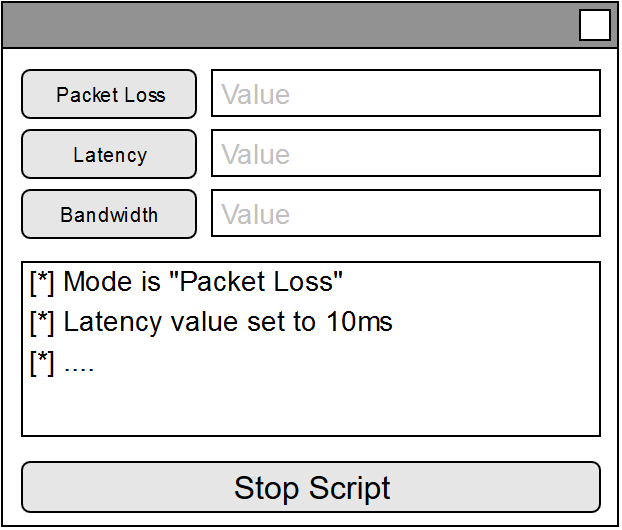
\includegraphics[scale=\imageScale]{Packet_UI_Design}};
	\node(GUIText)[below of=GUI, yshift=-0.5cm]{GUI};	
	
	\node(CLI)[base, below of=GUI, yshift=-2.25cm]{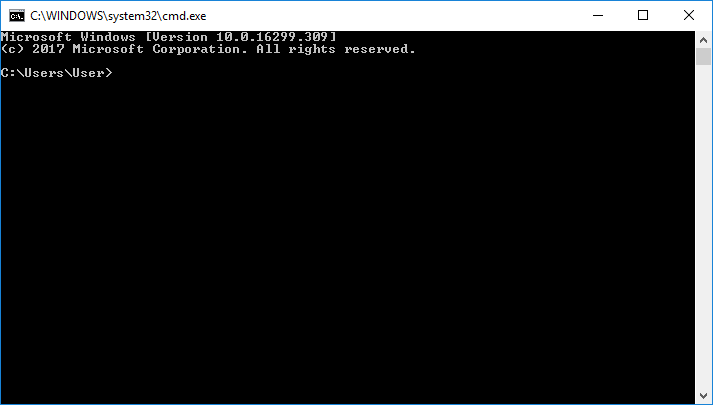
\includegraphics[scale=\imageScale]{CLI}};
	\node(CLIText)[below of=CLI]{CLI};
	
	\node(Effect)[blue, right of=User, xshift=(\width * 2) + 2cm]{Effect Choice};	
	\node(Nfqueue)[base, right of=Effect, xshift=(\width)]{NFQUEUE Creation};	
	
	\node(Parameters)[base, below of=Effect]{Parameter Handling};	
		
	
	\node(Packet)[red, below of=User, xshift=2cm, yshift=-4cm, text width=6cm]{Incomming Packets pushed into the NFQUEUE};
	\node(ChosenEffect)[blue, right of=Packet, xshift=\width + 2cm]{Chosen Effect};
	\node(PacketDescription)[above of=Packet, yshift=-0.5cm]{{\bf While NFQUEUE is running}};
	
	\draw[->] (User)--(GUI);
	\draw[->] (User)--(CLI);
	
	\draw[->] (GUI)--(Effect);
	\draw[->] (CLI)--(Parameters);
	\draw[->] (Parameters)--(Effect);	
	
	\draw[->] (Effect)--(Nfqueue);
	\draw[->] (Packet)--(ChosenEffect);
		
\end{tikzpicture}
\end{center}
	\begin{figure}[h]
		\caption{Architecture of the overall degradation tool}
	\end{figure}
\end{center}

It was decided early on that the script was to be controlled by two forms of interfaces; Graphical User Interface (GUI) and a text based Command Line Interface (CLI). This was to allow the tool to be run on the router (CLI) and also run on separate machines (GUI or CLI), this makes the tool versatile to many situations.

The system design is split into two stages:

\begin{itemize}
\item {\bf NFQUEUE Setup}\\
This section involves the creation of the NFQUEUE object, the binding of effect method to the queue and initialisation of variables dictating preferences.

\item {\bf NFQUEUE Running}\\
Each packet that is placed into the queue triggers this section, the handler is called that assigns a task to run the selected effect on the packet to one of the worker threads in a previously created thread pool. This allows custom effects alongside filtering can be dynamically applied to all the packets.
\end{itemize}

\subsection{Parameter Handling}
Parameter handling is only required on the CLI due to the unrestricted input of the interface. Below is the activity diagram for the parameter handling process:

\begin{center}
	\newcommand{\widthParameter}{4cm}

\tikzset{%
	>={Latex[width=2mm,length=2mm]},
	% Specifications for style of nodes:
            base/.style = {draw=black,
                           minimum width=\widthParameter, 
                           text width=\widthParameter, 
                           minimum height=1cm, 
                           text centered},                           
            decision/.style = {base, diamond, fill=yellow!15},
            normal/.style = {base, rectangle, rounded corners}}

\begin{tikzpicture}

	\node (start) [shape=circle, fill=black]{};
	
	\node (command) [normal, right of=start, xshift=\widthParameter]{Command is entered};
	\node (parse) [normal, right of=command, xshift=\widthParameter]{Parameters are parsed};
	
	\node (correctParam) [decision, below of=parse, yshift=\widthParameter * -1]{Parameters Correct?};
	\node (showUsage) [normal, below of=correctParam, yshift=-\widthParameter, fill=red!15]{Show Usage and quit};
	\node (saveParam) [normal, left of=correctParam, xshift=-\widthParameter * 2]{Call coresponding argument method with arguments};

	\node (end) [shape=circle, fill=black, below of=saveParam, yshift=-\widthParameter]{};

	\draw[->] (start)--(command);
	\draw[->] (command)--(parse);
	\draw[->] (parse)--(correctParam);
	
	\draw[->] (correctParam)--node[fill=white]{No}(showUsage);
	\draw[->] (correctParam)--node[fill=white]{Yes}(saveParam);
	
	\draw[->] (saveParam)--(end);
	\draw[->] (showUsage)--(end);

\end{tikzpicture}
	\begin{figure}[h]
		\caption{UML Activity Diagram for parsing and handling parameters}
	\end{figure}	
\end{center}

The parameter handling as stated previously is only required if the command line interface is used, this adds a little overhead in processing when using the command line but it is an unavoidable process. The error section when the `Usage' is printed will stop the entire program from continuing and will print a structured help message with the required format of the command. For most errors human readable output will be produces the aid in the debugging of the entered command.

\subsection{Effect Choice \& NQUEUE Creation}

\begin{center}
	\newcommand{\widthEffectChoice}{4cm}

\tikzset{%
	>={Latex[width=2mm,length=2mm]},
	% Specifications for style of nodes:
            base/.style = {draw=black,
                           minimum width=\widthEffectChoice, 
                           text width=\widthEffectChoice, 
                           minimum height=1cm, 
                           text centered},                           
            decision/.style = {base, diamond, fill=yellow!15},
            normal/.style = {base, rectangle, rounded corners}}

\begin{tikzpicture}

	\node (start) [shape=circle, fill=black]{};
	
	\node (setQueue) [right of=start, normal, xshift=\widthEffectChoice]
	{Binds the NFQUEUE's `Mode' to chosen effect};
	
	\node (setVariables) [right of=setQueue, normal, xshift=\widthEffectChoice]
	{Sets all \\ preference \\ variables by parsed \\ arguments};
	
	\node (userOutput) [fill=blue!15, below of=setVariables, normal, yshift=-\widthEffectChoice + 2cm]
	{Displays summary of chosen modes and prefrences to the user};
	
	\node (runNfqueue) [left of=userOutput, normal, xshift=-\widthEffectChoice]
	{NFQUEUE Object is then run. That will pass all packets to the assigned 'Mode'};

	\node (end) [shape=circle, fill=black, below of=start, yshift=-\widthEffectChoice + 2cm]{};

	%Arrows
	\draw[->] (start)--(setQueue);
	\draw[->] (setQueue)--(setVariables);
	\draw[->] (setVariables)--(userOutput);
	\draw[->] (userOutput)--(runNfqueue);
	\draw[->] (runNfqueue)--(end);

\end{tikzpicture}
	\begin{figure}[h]
		\caption{UML Activity Diagram for assigning the choice of effect}
	\end{figure}
\end{center}


Choosing a mode for the program gives the ability to switch between degradation effect and arrangement of effects. This process is exactly the same for GUI and CLI. This is due to the shared code between the different user interfaces, all the CLI does is add a wrapper on top that allows control of the concealed code by the way of parsed arguments and the GUI just directly calls these methods when buttons are clicked.

\subsection{Incoming Packets}
\begin{center}
	\begin{tikzpicture}

	\node (start) [shape=circle, fill=black]{};
	
	\node (handler) [normal, right of=start, xshift=\width * 2] 
	{Packet placed into queue caught by handler method};
	
	\node (filterSet) [below of=handler, yshift=-\width, decision] {Is packet filter set?};
	\node (targetCheck) [left of=filterSet, xshift=-\width * 2, normal]{Check filter against packet};
	\node (passFilter) [below of=targetCheck, yshift=-\width, decision]{Does packet pass filter};
	
	\node (runEffect) [below of=filterSet, yshift=-\width, normal, fill=red!15]
	{Run assigned \\ effect on packet};	
	
	\node (Accept) 	[fill=blue!15, below of=passFilter, normal, yshift=-\width]{Accept Packet};
	\node (Drop)	[fill=blue!15, below of=runEffect, normal, yshift=-\width]{Drop Packet};	
	
	%Find the middle between the two nodes
 	\coordinate (CENTER) at ($(Accept)!0.5!(Drop)$);		
	\node (end)	[below of=CENTER, shape=circle, fill=black, yshift=-2cm]{};	
	
	\node (endLabel) [below of=end]{Thread released};	
	
	% Connections
	\draw[->] (start)--(handler);
	\draw[->] (handler)--(filterSet);
	
	\draw[->] (filterSet)--node[fill=white]{Yes}(targetCheck);
	\draw[->] (filterSet)--node[fill=white]{No}(runEffect);
	
	\draw[->] (targetCheck)--(passFilter);
	
	\draw[->] (passFilter)--node[fill=white]{Yes}(runEffect);
	\draw[->] (passFilter)--node[fill=white]{No}(Accept);	

	\draw[->] (runEffect)--(Accept);
	\draw[->] (runEffect)--(Drop);
	
	\draw[->] (Drop)--(end);
	\draw[->] (Accept)--(end);	
s
\end{tikzpicture}
	\begin{figure}[h]
		\caption{Activity diagram for running an effect on a single packet}
	\end{figure}
\end{center}

Above is the activity diagram for the process of running an effect on a single packet. The script automatically effects every packet that is placed in the NFQUEUE, this means protocol support does not need to be managed and no code manipulating or monitoring sockets is required.

% Section Description:
%
\section{Tool Class Design}
\subsection{Effect Class Diagram}

\begin{center}
	\begin{tikzpicture}

% Effect - Parent class
\umlclass{Effect}
{
	+ allow\_print 		: bool \\ 
	+ accept\_packets 	: bool
}
{
	+ print()			: void \\
	+ print\_stats()	: void \\
	+ effect()			: void 	
}

\umlclass[below right= 2cm of Effect]{Latency}
{
	+ latency\_value\_ms : int
}

\umlclass[below = 1.45cm of Effect]{PacketLoss}
{
	+ packet\_loss : int
}

\umlclass[below left= 2cm of Effect]{Bandwidth}
{
	+ rate\_limit : int
}

% Links
\umlVHVinherit{Effect}{Latency}
\umlVHVinherit{Effect}{PacketLoss}
\umlVHVinherit{Effect}{Bandwidth}

\end{tikzpicture}
	\begin{figure}[h]
		\caption{UML Class diagram for producing degradation effects}
	\end{figure}
\end{center}

The above design is for the various effects that will be implemented into the program. They will be self contained within separate modules encased in an object. This was chosen so each effect is modular and self contained from one another, this will improve the potential readability and maintainability of the code base, it will also make the code base much more scalable where effects can be added with high speed because of the lack of repeated code.  Each effect will inherit from the base class ``Effect", where it will obtain method and properties used for functionality, boolean variables for allowing printing and accepting packets, these are both necessary when `chaining' effects together, where a packet can only be accepted once and only a single print will be required.

\subsection{Effect Activity Diagram}
\begin{center}
	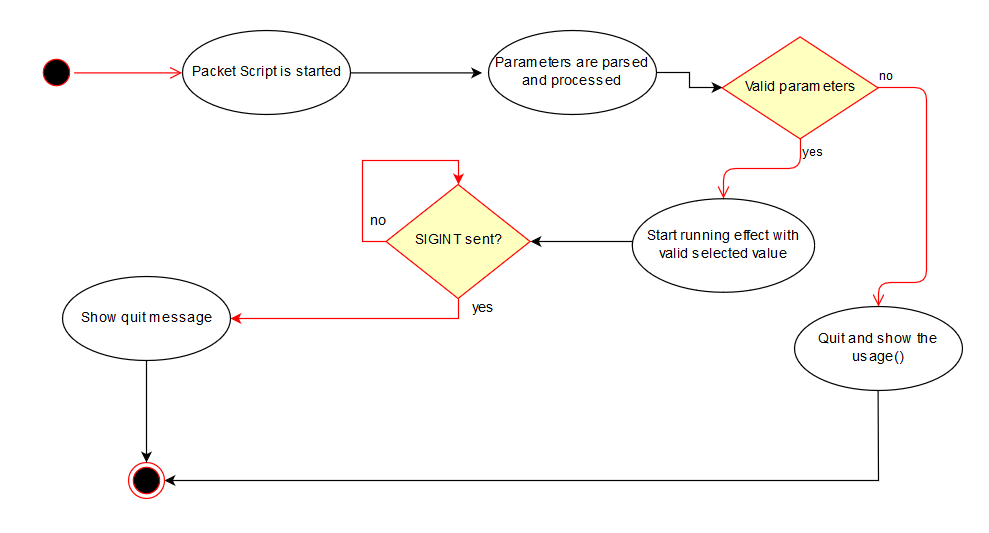
\includegraphics[scale=0.6]{Packet_Activity_Diagram}
	\begin{figure}[h]
		\caption{Activity Diagram for the degradation script}
	\end{figure}
\end{center}

Above is the activity diagram for the packet script that will implement the effect classes above, this script will be utilised directly from the command line or run by the GUI. The decision of having a single script that is controlled by multiple ways allow for one central point of functionality and means code can be shared throughout the project. The activity diagram shows the design choices for the direct control on the script. SIGINT is mentioned in the centre of the diagram, SIGINT is a built in signal in the Linux operating system that represents an interrupt signal, where it is triggered by pressing ``Control + C", this is the most common/clean way of stopping a script. The other alternatives to closing the script ``Control + Z" (SIGTSTP) and ``Control + /" (SIGQUIT) will be remapped to send a SIGINT signal and perform the same role, this will mean the program has one tidy point of closure.




% Section Description:
%
\section{Tool UI Design}
One of the ways mentioned before to control the degradation effects is by a user interface. It needs to have a way to easily add new buttons and text entries that link up to parameters in the script to make the interface scalable and easy to maintain, it also needs a window to display the same output as the terminal window, this can be achieved by `piping' the stdout to a custom section of the user interface. The `stdout' is the data stream that links up to a Linux terminal window, if the stdout points to somewhere else it will display where it is needed. Below is the initial drafted design for the user interface.

\begin{center}
	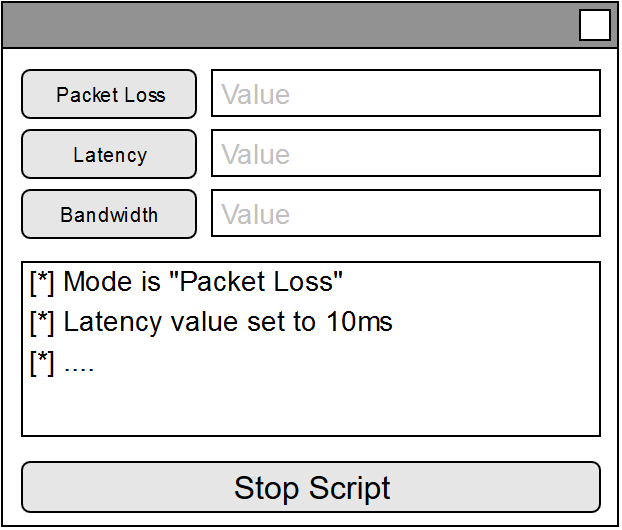
\includegraphics[scale=0.5]{Packet_UI_Design}
	\begin{figure}[h]
		\caption{Initial user interface design for the Degradation GUI}
	\end{figure}
\end{center}



% Section Description:
%
\section{Tool Implementation}

\subsection{NFQUEUE}
The script utilises a section in the Linux kernel referred to as the ``NFQUEUE". This is as the name suggests a queue that is stored in kernel memory that will store up packets until the user provides one of the two verdicts: `Drop' or `Accept'. The packets are pushed into this queue by the use of `iptable' rules, iptabales is a tool designed to filter packets by criteria. Below is a flow diagram for the path a packet might take, each table can have filtering rules embedded into to it:

% Diagram
%Variables
\newcommand{\nodefont}{\rmfamily}
\newcommand{\normalWidth}{3cm}

%----------------------------------------%
%  IPtables Diagram						 %
%----------------------------------------%
\tikzset{%
  >={Latex[width=2mm,length=2mm]},
  % Specifications for style of nodes:
            base/.style = {rectangle, rounded corners, draw=black,
                           minimum width=4cm, minimum height=1cm,
                           text centered, font=\sffamily}, 
            process/.style = {base, minimum width=\normalWidth, fill=orange!15,
                           font=\nodefont},
            network/.style = {base, fill=blue!15},
            local/.style = {base, fill=red!15}}
\vspace{0.25cm}                
\begin{center}
\begin{tikzpicture}[node distance=1.5cm, every node/.style={fill=white, font=\sffamily}, align=center]
    	\node(NetworkCard)[network]{Network Card};
        \node(NetworkCardOut)[network, right of=NetworkCard, xshift=6cm]{Network Card};
        
    	\node(PreRouting)[process, below of=NetworkCard]{Pre-Routing};
    	\node(Forward)[process, right of=PreRouting, xshift=2.5cm, yshift=-1.75cm]{Forward};
    	\node(Input)[process, below of=PreRouting, yshift=-2cm]{Input};
        \node(PostRouting)[process, right of=PreRouting, xshift=6cm]{Post-Routing};
    	\node(Output)[process, right of=Input, xshift=6cm]{Output};
        
        \node(LocalProcessIn)[local, below of=Input]{Local Process};
        \node(LocalProcessOut)[local, below of=Output]{Local Process};
        
        %In Arrows
        \draw[->] (NetworkCard)--(PreRouting);
        \draw[->] (PreRouting)|-(Forward);
        \draw[->] (PreRouting)--(Input);
        \draw[->] (Input)--(LocalProcessIn);
        
        %Out Arrows
        \draw[->] (LocalProcessOut)--(Output);
        \draw[->] (Output)--(PostRouting);
        \draw[->] (Forward)-|(PostRouting);
        \draw[->] (PostRouting)--(NetworkCardOut);        
\end{tikzpicture}
\end{center}   

If there was a case where all packets entering the machine need filtering, an iptable rule would be added to the "Pre-Routing" section of the table to catch all packets entering the machine. 

So for example to move all packets entering from the network card into the NFQUEUE the iptable rule would be added like so:
\begin{center}
	\begin{console_font}
		\large{iptables -A INPUT -j NFQUEUE}
	\end{console_font} 
\end{center}
Where `-a' tells to append a rule onto the `INPUT' table and `-j' is the rule that affects the packet, in this case pushing it into the default queue.

This forms the main component of the functionality of the script, a series of iptable rules that filter packets into the NFQUEUE and allow to script to perform verdicts on each packet separately allows for effects to be easily applied to packets entering and leaving the machine.



The NFQUEUE is created like so: 
\begin{center}
\begin{Code}[]{NFQUEUE Creation}
# Setup for the NQUEUE
nfqueue = NetfilterQueue()

try:
	nfqueue.bind(0, mode)  # 0 is the default NFQUEUE
except OSError:
	print_force("[!] Queue already created")
\end{Code}
\end{center}

\subsection{Degradation Effects}
The script contains the functionality to simulate a plethora of effects and each effects functionality will be described below. Please not any of these effects can be chained together in any order.

\subsubsection{Latency}
Latency as described in the background section is the delay in initiating a task and seeing its results. Latency is simulated by using a timing mechanisms where the arrival time of the packet is saved. The packet is then pushed into the NFQUEUE that triggers a single thread that will hold the packet for a set amount of time, the holding time is calculated by taking the amount of time the packet has already been in the script away from the target time. The packet is then marked as `ACCEPTED' and pushed out of the queue.

\subsubsection{Packet Loss}
Packet loss is simulated by first assigning a target value, lets say for this example 10\%. For each packet the script randomly generates a number between 1 and 100, if that value is less than the target value the packet is dropped, and if the value is larger the packet is accepted. This therefore creates the effect of packet loss. It does however require a fair amount of packets to balance out statistically and reach the percentage target.

\subsubsection{Bandwidth}
There are two modes created for bandwidth; rate limiting and a simple display. Rate limiting allows the script to limit the rate of bandwidth flowing through the machine and calculates the rate transferred over a period of 5 seconds, if the rate is higher it waits until the rate drops below the target. This gives it the ability to adjust quickly and allows the script to be run for a long period of time without the overall average of the bandwidth affecting future changes. Displaying the bandwidth work exactly the same but without the limit check, this is useful when checking the current download speeds or the max transfer rate.

\subsubsection{Out-of-order}
This effect changes the order of packets coming into the script, this can be used to check its effect on UDP and TCP and can test how quickly these issue can be rectified. It works by queuing up every packet into a list, then a single thread randomly picks an index of that list, accepts the packet and allows it to leave. This therefore means at its most extreme the order can be last in, first out.

\subsubsection{Connection Simulation}
Connection simulation isn't quite a degradation effect but its intent is to simulate the effect of degradation on a common connection like `WiFi` or a 3G connection to see how these are effected by said degradation. This can be useful in some situations where for example testing a mobile applications performance over 3G with heavy latency, the mobile would connect to the script and the script would effect any traffic entering or leaving the handset.

\subsubsection{Jitter}
Jitter mode clumps and separates packets in their transmission, with some it waits a small period of time other it will clump up delay as a total and then send them all at once. This is to test how the protocol deals with jitter in the connection. Jitter as explained in the background is the intra-packet latency i.e. the difference in time between arrivals of packets.

\subsection{ARP Spoofing}
The script also supports an ARP spoofing mode that allows it to sit between a gateway and a specified target. This means the script can perform all its functions on a single target with a very quick deployment time. As touched on in the background the ARP protocol performs no authentication on any changes to the ARP cache meaning that you can perform a man in the middle attack and route traffic through a machine of your choice.

The script begins by grabbing the MAC addresses connected to the provided gateway and target IP addresses. Two ARP reply packets (denote by the `2' opcode) are sent out: One telling the victim that the current machines MAC address maps to the gateway, and the other telling the gateway that the victims IP maps to the current machines MAC address.

Below is the process visualised:




% Gateway
\newcommand{\GatewayLabel}{
\begin{tabular}{l l}
Gateway\\
\hline
\vspace{0.1cm}
\bf{192.168.1.1} & \bf{C8:49:BD:82:47:4D}\\
ARP Cache\\
\hline
192.168.1.2 & 46:41:73:EC:70:E3
\end{tabular}
}

%Victim
\newcommand{\VictimLabel}{
\begin{tabular}{l l}
Victim\\
\hline
\vspace{0.1cm}
\bf{192.168.1.2} & \bf{46:41:73:EC:70:E3}\\
ARP Cache\\
\hline
192.168.1.1 & C8:49:BD:82:47:4D
\end{tabular}
}

\begin{center}
\begin{tikzpicture}[
    diagram item/.style={},
    align=left
]         

\node (Router)[
    diagram item,
    label=above:\GatewayLabel,
    yshift=-2cm
] {
\includegraphics[scale=\ciscoImageScale]{\cisco/router}};

\node (Victim)[
	diagram item,
	label=above:\VictimLabel,
	right of=Router,
	xshift=7cm
] {
\includegraphics[scale=\ciscoImageScale]{\cisco/workstation}};


\draw[-] (Router)--(Victim);

\end{tikzpicture} 
\end{center}


As you can see both ends are connected and have gone through the process to resolve the IP addresses to MAC addresses, you can see above each device their corresponding IP, MAC and ARP Cache. The ARP cache as mentioned previously is a record linking IP addresses to MAC addresses.

\newcommand{\tgap}{0.1cm}

% Gateway
\newcommand{\GatewayLabelAfter}{
\begin{tabular}{l l}
Gateway\\
\hline
\vspace{\tgap}
\bf{192.168.1.1} & \bf{C8:49:BD:82:47:4D}\\
ARP Cache\\
\hline
192.168.1.2 & \bf{\textcolor{red}{37:A8:22:F6:BB:34}} \\
192.168.1.3 & 37:A8:22:F6:BB:34
\end{tabular}
}

%Victim
\newcommand{\VictimLabelAfter}{
\begin{tabular}{l l}
Victim\\
\hline
\vspace{\tgap}
\bf{192.168.1.2} & \bf{46:41:73:EC:70:E3}\\
ARP Cache\\
\hline
192.168.1.1 & \bf{\textcolor{red}{37:A8:22:F6:BB:34}} \\
192.168.1.3 & 37:A8:22:F6:BB:34
\end{tabular}
}

%Attacker
\newcommand{\AttackerLabel}{
\begin{tabular}{l l}
Attacker\\
\hline
\bf{192.168.1.3} & \bf{37:A8:22:F6:BB:34} 
\end{tabular}
}

\begin{center}
\begin{tikzpicture}[
    diagram item/.style={},
    align=left
]         

\node (Router)[
    diagram item,
    label=above:\GatewayLabelAfter,
    yshift=-2cm
] {
\includegraphics[scale=\ciscoImageScale]{\cisco/router}};

\node (Victim)[
	diagram item,
	label=above:\VictimLabelAfter,
	right of=Router,
	xshift=7cm
] {
\includegraphics[scale=\ciscoImageScale]{\cisco/workstation}};


%Find the middle between the two nodes
\coordinate (CENTER) at ($(Victim)!0.5!(Router)$);		
\node (Attacker)[
	label=below:\AttackerLabel,
	below of=CENTER,
	yshift=-3.5cm
] {
\includegraphics[scale=\ciscoImageScale]{\cisco/laptop}};

\draw[red, very thick] (Router)--(Attacker);
\draw[red, very thick] (Attacker)--(Victim);


\end{tikzpicture} 
\end{center}


Note after the 3rd device connects to the network, both devices gain a record of its IP and MAC address in their ARP cache. 

After both spoofed packets have been send out the ARP cache for each receiving end gets updated, the text in red shows the changes caused by the spoofed ARP packets. Now when either end wants to talk to each other it will resolve the MAC address and send it with the new MAC address in the table, this will therefore get routed through the attacking PC and will allow the script to receive all the traffic between the two parties.

\subsection{Network Attacks}
A couple of network attacks were implemented into the script, these served the purpose of providing very heavy artificial traffic designed to create heavy loads or mess with integral protocols. Not many attacks were added as they don't provide much purpose apart from stress testing and they reside on the edge of the scope of this project. There will also be a brief discussion into possible techniques to mitigate the effects. 

\subsubsection{UDP Flooding}
UDP flooding is a very simple attack, lots of UDP packets are created and send over a network stream very quickly. This attack is designed to `flood' the buffers in the receiving machine and slow down or event prevent internet connection. The script creates 10 or so threads that create and send packet concurrently, this amount of threads easily reaches the max throughput of the test machines NIC card and massively reduces internet connection on the receiving end.

The attack could be detected and prevented by a script that monitors the network transfers rates, this attack will create a huge spike in the transfer rate that can be detected and all traffic would be blocked from the sending party.

\subsubsection{ARP Spamming}
This attack works by once again exploiting the lack of authentication of the ARP protocol. In the entire network mode the script starts by detecting all active hosts on a network, it then starts sending out falsified ARP reply packets with randomly generated MAC addresses inside. This results in all computers on the networking having incorrect ARP cache values and resulting in computers incorrectly resolving IP and MAC address combinations and traffic not being allowed through.

This attack is relatively easy to execute but can simply be prevented by issuing static ARP tables for each machine, this prevents unsolicited ARP replies from changing IP and MAC address combinations and also prevents ARP Spoofing from occurring on that network.


%Experimental design:
%If you project includes any experiments, including but not limited to user testing, then you can discuss their design here. Note that again this does not exist in a vacuum and should be tied to your research.

\section{Test design and system testing}
There are various sections of the project that require a separate testing plan:

\begin{itemize}

	\item Traffic simulation programs\\
	These are the client server programs that will simulate traffic over the synthetic net. These tests will need to 	make 	sure each client and server performs its role correctly.
	
	\item Packet script and effects\\
	This is the script that will run on the custom router. Tests will be checking effects do their basic jobs and the script can be controlled effectively.
	
\end{itemize}

\subsection{Traffic simulation programs}
The test plan for this section will need to check all the intended functionality of each window. There are three aspects of each that will need testing:

\begin{itemize}

	\item UI \\
	Tests will be created that click buttons and check the user interface works effectively through automated testing.

	\item Business Logic \\
	Code behind the UI will have the relevant methods testing with expected and actual results.

	\item Real world usage \\
	The involvement of multiple windows and more complex functionality can be tested by using automated testing 			scripts.
	
\end{itemize}

Appendix A contains the test plan for the program, each separate program has had its user interface and business logic tested and programs that are to be used together have had ``Live" tests created to check their interaction together. The automated tests have been achieved by using the CUIT (Coded User Interface Tests) \footnote{\url{https://msdn.microsoft.com/en-us/library/dd286726.aspx}} that are built into Visual Studio 2017. These allow clicks and movements to be recorded and repeated.

\subsection{Packet Script}
It was decided that a separate test plan was needed for the script that will be run on the router. This was because its design is considerably different to that of the traffic simulation programs. Each individual effect needs a basic test that uses a loopback ping test to simulate incoming traffic where a criteria is looked for, for example to test packet loss, the test pings the script until a packet is lost or a time-out is reached, this can perform a basic test on the functionality of the effect. Each effect will also require validation for the passed parameters, there will be a test created that will test various values inside and outside of the validation range.

\subsection{Testing methodology considerations}
Initially the methodology chosen to start development of the traffic simulation programs was ``Test Driven Development" \citep{beck2003test}, this was a tight methodology that increased development time and gave the added benefit of showing that new changes have not broken older functionality. This methodology was good to start off the project and allowed for a tight structure to be created where no time was wasted debugging previously working code, but as mentioned this methodology slowed development time down, this was chosen to be abandoned after 3-4 weeks to an ad-hoc approach. 
This change was due to time restraints on the project and the less-important role that the traffic simulation programs had on the project compared to the degradation simulation script. The degradation script was developed in the ad-hoc approach, this was due to issue stated previously about the unknown aspects of the script and how it would be operating that it was decided that the time invested to write up test scripts would assume too much and would risk them having the be completely rewritten, tests therefore was added alongside new functionality.





% Section Description
%
\section{Experiential design}
\subsection{Latency Accuracy}
In the initial stages of the project there were experiments that tested the effects of the degradation on the network, the tests were performed on the loopback (Internal network 127.0.0.1) with ICMP ping packets.

This test was designed to show the accuracy of different ways of simulating latency, the first way being a static timer that just causes the thread to sleep for a set amount of time or a dynamic timer that calculates the elapsed time since the creation of the thread and the command telling the thread to sleep, the dynamic timer takes this elapsed time off the target latency value.

Below the results are visualised in a single graph. Please note - the relatively high percentage error in the small ranges of latency this is due to the error proportion being a much larger chunk of the overall target latency and therefore being a higher percentage error:

\begin{tikzpicture}[every axis plot/.append style={thick}]
		\begin{axis}[
			width=\linewidth,
			height=10cm,
			grid=major,
			xmin=1, xmax=100,
			ymin=0, ymax=100,
			xlabel=Latency (ms),
			ylabel=Error (\%)]
			\addplot table [x index=0, y index=1, mark=none, search path=csv_data, col sep=comma]{PingTestDynamicVsStatic.csv};		
			\addlegendentry{Static}	
			
			\addplot table [x index=0, y index=2, mark=none, search path=csv_data, col sep=comma]{PingTestDynamicVsStatic.csv};		
			\addlegendentry{Dynamic}	
		 \end{axis}
 \end{tikzpicture}
 

As you can see from the graph the dynamic form of issuing latency is overall more accurate in simulation, but however, it is still not perfect and there seems to be a small overall error present. This performance is however more than suitable for the scope of this project.

\subsection{Visualising effects}
The most effective way to visualise real world connections were running tests on SpeedTest.net \footnote{\url{http://beta.speedtest.net/}}. This is very useful to quickly visualise a certain effect on the network.

Below are two images showing the effect of a 100ms latency on a networks speed. Both tests were performed on the same empty network and the best result was taken from 5 runs on each.

\begin{center}
	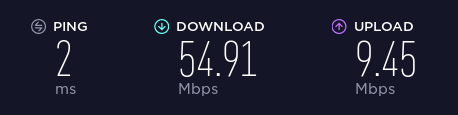
\includegraphics[scale=0.5]{SpeedNoEffect}
	\begin{figure}[h]
		\caption{The initial connection speed}
	\end{figure}
\end{center}

\begin{center}
	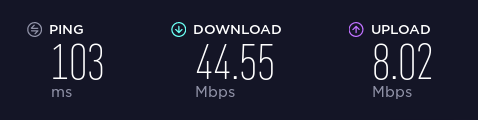
\includegraphics[scale=0.5]{Speed100ms}
	\begin{figure}[h]
		\caption{Network speed with a latency of 100m/s}
	\end{figure}
\end{center}

As you can see from both images, the 100ms has evidently been applied effectively and the speed of the connection has dropped by around 10Mbps. This means in real world terms the time taken to download a 1GB file would take 35 seconds longer to download. This is not a considerable reduction but the latency is having a obvious effect on the network quality.